% !TeX program = pdfLaTeX
\documentclass[aoas]{imsart}
\usepackage{amsmath,amsfonts,amssymb}
\usepackage{graphicx}
\usepackage[round,sort&compress]{natbib}
\usepackage[letterpaper=true,colorlinks=true,pdfpagemode=none,urlcolor=blue,linkcolor=blue,citecolor=blue,pdfstartview=FitH]{hyperref}
\usepackage{color}
\usepackage{booktabs}


\usepackage{algorithm,algorithmic}
\def\algorithmautorefname{Algorithm}


\renewcommand*{\figureautorefname}{Figure}%
\renewcommand*{\tableautorefname}{Table}%
\renewcommand*{\partautorefname}{Part}%
\renewcommand*{\chapterautorefname}{Chapter}%
\renewcommand*{\sectionautorefname}{Section}%
\renewcommand*{\subsectionautorefname}{Section}%
\renewcommand*{\subsubsectionautorefname}{Section}%

\usepackage{wasysym}


\usepackage{xr}
\externaldocument{aoas/musicManuscript-rev1}

%% load any required packages here




% Number only ref'ed equations
\usepackage{mathtools}
\mathtoolsset{showonlyrefs,showmanualtags}

\renewcommand{\algorithmiccomment}[1]{\hfill $\rhd$ #1}
\renewcommand{\thealgorithm}{A\arabic{algorithm}} 

\usepackage{afterpage}

\renewcommand\thefigure{SM-\arabic{figure}}
\newcommand{\email}[1]{\href{mailto:#1}{#1}}

%\usepackage{setspace}

\newcommand{\norm}[1]{\left\lVert #1 \right\rVert}
\renewcommand{\hat}{\widehat}
% next three lines to give Kalman filter sample \varx_t=E[x_t|y_1,...,y_t]
\usepackage{upgreek}
\DeclareRobustCommand{\varx}{{\mathpalette\irchi\relax}}
\newcommand{\irchi}[2]{\protect\raisebox{\depth}{$#1\upchi$}}
\newcommand{\given}{\ \vert\ }
\newcommand{\E}{\mathbb{E}}
\newcommand{\Expect}[1]{\E\left[#1\right]}
\newcommand{\Var}[1]{\mathbb{V}\left[#1\right]}
\newcommand{\indicator}[1]{\boldsymbol{1}\left(#1\right)}

\begin{document}

\begin{frontmatter}
  
\title{Supplement to Markov-Switching State Space Models for Uncovering Musical
  Interpretation}
\runtitle{Supplement to Switching Models for Music}
\author[AA]{%
  \fnms{Daniel J.} \snm{McDonald}\corref{}\ead[label=ee1]{daniel@stat.ubc.ca}},
\author[BB]{%
  \fnms{Michael} \snm{McBride}\ead[label=ee2,mark]{michmcbr@iu.edu}},
\author[CC]{%
  \fnms{Yupeng} \snm{Gu}\ead[label=ee3,mark]{yupeng.gu@gmail.com}},
\and
\author[CC]{\fnms{Christopher} \snm{Raphael}\ead[label=ee4,mark]{craphael@indiana.edu}}

\runauthor{McDonald, McBride, Gu, and Raphael}
\address[AA]{Department of
  Statistics, University of British Columbia, \printead{ee1}}
\address[BB]{Department of
  Statistics, Indiana University, \printead{ee2}}
\address[CC]{School of Informatics,
  Computing, and Engineering, Indiana University, \printead{ee3,ee4}}

\end{frontmatter}




\hypertarget{algorithms}{%
\section{Algorithms}\label{algorithms}}

For completeness, we include here concise descriptions of the Kalman
filter and smoother we employ as inputs to our main algorithm. The
filter is given in \autoref{alg:kalman}.

\begin{algorithm}
  \caption{Kalman filter: estimate $x_i$ conditional on
    $\{y_j\}_{j=1}^i$, for all $i=1,\ldots,n$ and calculate the log likelihood
    for $\theta$\label{alg:kalman}}
  \begin{algorithmic}
    \STATE {\bf Input:} $Y$, $x_0$, $P_0$, $d,\ T,\ c,\ Z,$ and $G$
    \STATE $\ell(\theta) \leftarrow 0$ \COMMENT{Initialize the log-likelihood}
    \FOR{$i=1$ to  $n$}
    \STATE $\begin{aligned}\varx_{i}
      &\leftarrow d + T x_{i-1|i-1}, & P_i &\leftarrow Q + T P_{i-1|i-1}
      T^\top\end{aligned}$ \COMMENT{Predict current state}
    \STATE $\begin{aligned}\widetilde{y}_i
      &\leftarrow c + Z \varx_i, & F_i &\leftarrow G + Z P_i
      Z^\top\end{aligned}$ \COMMENT{Predict current observation}
    \STATE $\begin{aligned}v_i&\leftarrow y_i-\widetilde{y}_i& K_i&
      \leftarrow P_i Z^\top F^{-1}\end{aligned}$ \COMMENT{Forecast error and 
    Kalman gain}
    \STATE $\begin{aligned} x_{i|i}
      &\leftarrow \varx_i + K_i v_i, & P_{i|i} &\leftarrow P_i - P_iZ^\top
      K_i\end{aligned}$ \COMMENT{Update}
    \STATE $\ell(\theta) = \ell(\theta) -v_i^\top F^{-1}v_i - \log(|F_i|)$
    \ENDFOR
    \RETURN $\widetilde{Y}=\{\widetilde{y}_i\}_{i=1}^n,\ \varx=\{\varx_i\}_{i=1}^n,\
    \widetilde{X}=\{x_{i|i}\}_{i=1}^n,\ P=\{P_i\}_{i=1}^n,\
    \widetilde{P}=\{P_{i|i}\}_{i=1}^n,\ \ell(\theta)$
  \end{algorithmic}
\end{algorithm}

To incorporate all future observations into these estimates, the Kalman
smoother is required. There are many different smoother algorithms
tailored for different applications. \autoref{alg:kalman-smoother}, due
to \citet{RauchStriebel1965}, is often referred to as the classical
fixed-interval smoother \citep{AndersonMoore1979}. It produces only the
unconditional expectations of the hidden state
\(\hat{x}_i=\Expect{x_i\given y_1,\ldots,y_n}\) for the sake of
computational speed. This version is more appropriate for inference in
the type of switching models we discuss in the manuscript.

\begin{algorithm}
  \caption{Kalman smoother (Rauch-Tung-Striebel): estimate $\hat{X}$ conditional on
    $Y$\label{alg:kalman-smoother}} 
  \begin{algorithmic}
    \STATE {\bf Input:} $\varx$, $\widetilde{X}$, $P$, $\widetilde{P}$,
    $T,$ $c$, $Z$.
    \STATE $i=n$,
    \STATE $\hat{x}_{n}\leftarrow \widetilde{x}_n$, 
    \WHILE{$t>1$}
    \STATE $\hat{y}_i \leftarrow c + Z\hat{x}_i,$
    \COMMENT{Predict observation vector}
    \STATE $\begin{aligned} e &\leftarrow \hat{x}_i -
      \varx_i, & V &\leftarrow P_i^{-1}\end{aligned}$,
    \STATE $i\leftarrow i-1$, \COMMENT{Increment}
    \STATE $\hat{x}_i = \widetilde{x}_i + \widetilde{P}_i T Ve $ 
    \ENDWHILE
    \RETURN $\widehat{Y}=\{\hat{y}_i\}_{i=1}^n, \hat{X}=\{\hat{x}_i\}_{i=1}^n$
  \end{algorithmic}
\end{algorithm}

\hypertarget{principal-components}{%
\section{Principal components}\label{principal-components}}

In \autoref{sec:clust-music-perf} of the main document, we plotted the
first two principal components along with some notion of groups to gauge
the similarities between performances. \autoref{tab:lin-pc-loadings}
gives the loadings for the first three principal components. We see that
the first component picks up information about the first two states,
both through \(\mu_{\textrm{tempo}}\) and \(\mu_{\textrm{acc}}\) as well
as loading onto the probabilities \(p_{11}\), \(p_{12}\), and
\(p_{31}\). The second component loads especially onto
\(\mu_{\textrm{stress}}\) but also \(p_{11}\) and \(p_{21}\). Finally,
the third component loads mainly onto the observation error with smaller
contributions from \(p_{31}\).

\begin{table}

\caption{\label{tab:lin-pc-loadings}The factor loadings for principal component analysis of the parameter estimates.}
\centering
\resizebox{\linewidth}{!}{
\begin{tabular}[t]{lrrrrrrrrrrrr}
\toprule
  & $\sigma_\epsilon^2$ & $\mu_{\textrm{tempo}}$ & $\mu_{\textrm{acc}}$ & $\mu_{\textrm{stress}}$ & $\sigma_{\textrm{tempo}}^2$ & $p_{11}$ & $p_{12}$ & $p_{31}$ & $p_{13}$ & $p_{21}$ & $p_{32}$ & $p_{22}$\\
\midrule
PC1 & 0.07 & 0.34 & -0.66 & -0.22 & -0.09 & 0.27 & -0.34 & 0.32 & 0.03 & -0.05 & -0.3 & -0.05\\
PC2 & 0.07 & 0.00 & -0.12 & -0.48 & -0.02 & -0.46 & 0.13 & -0.01 & 0.17 & 0.68 & 0.0 & -0.17\\
PC3 & 0.64 & -0.59 & 0.16 & 0.02 & -0.03 & 0.08 & -0.13 & 0.32 & 0.03 & 0.05 & -0.3 & -0.02\\
\bottomrule
\end{tabular}}
\end{table}

\hypertarget{confidence-intervals}{%
\section{Confidence intervals}\label{confidence-intervals}}

\begin{figure}

{\centering 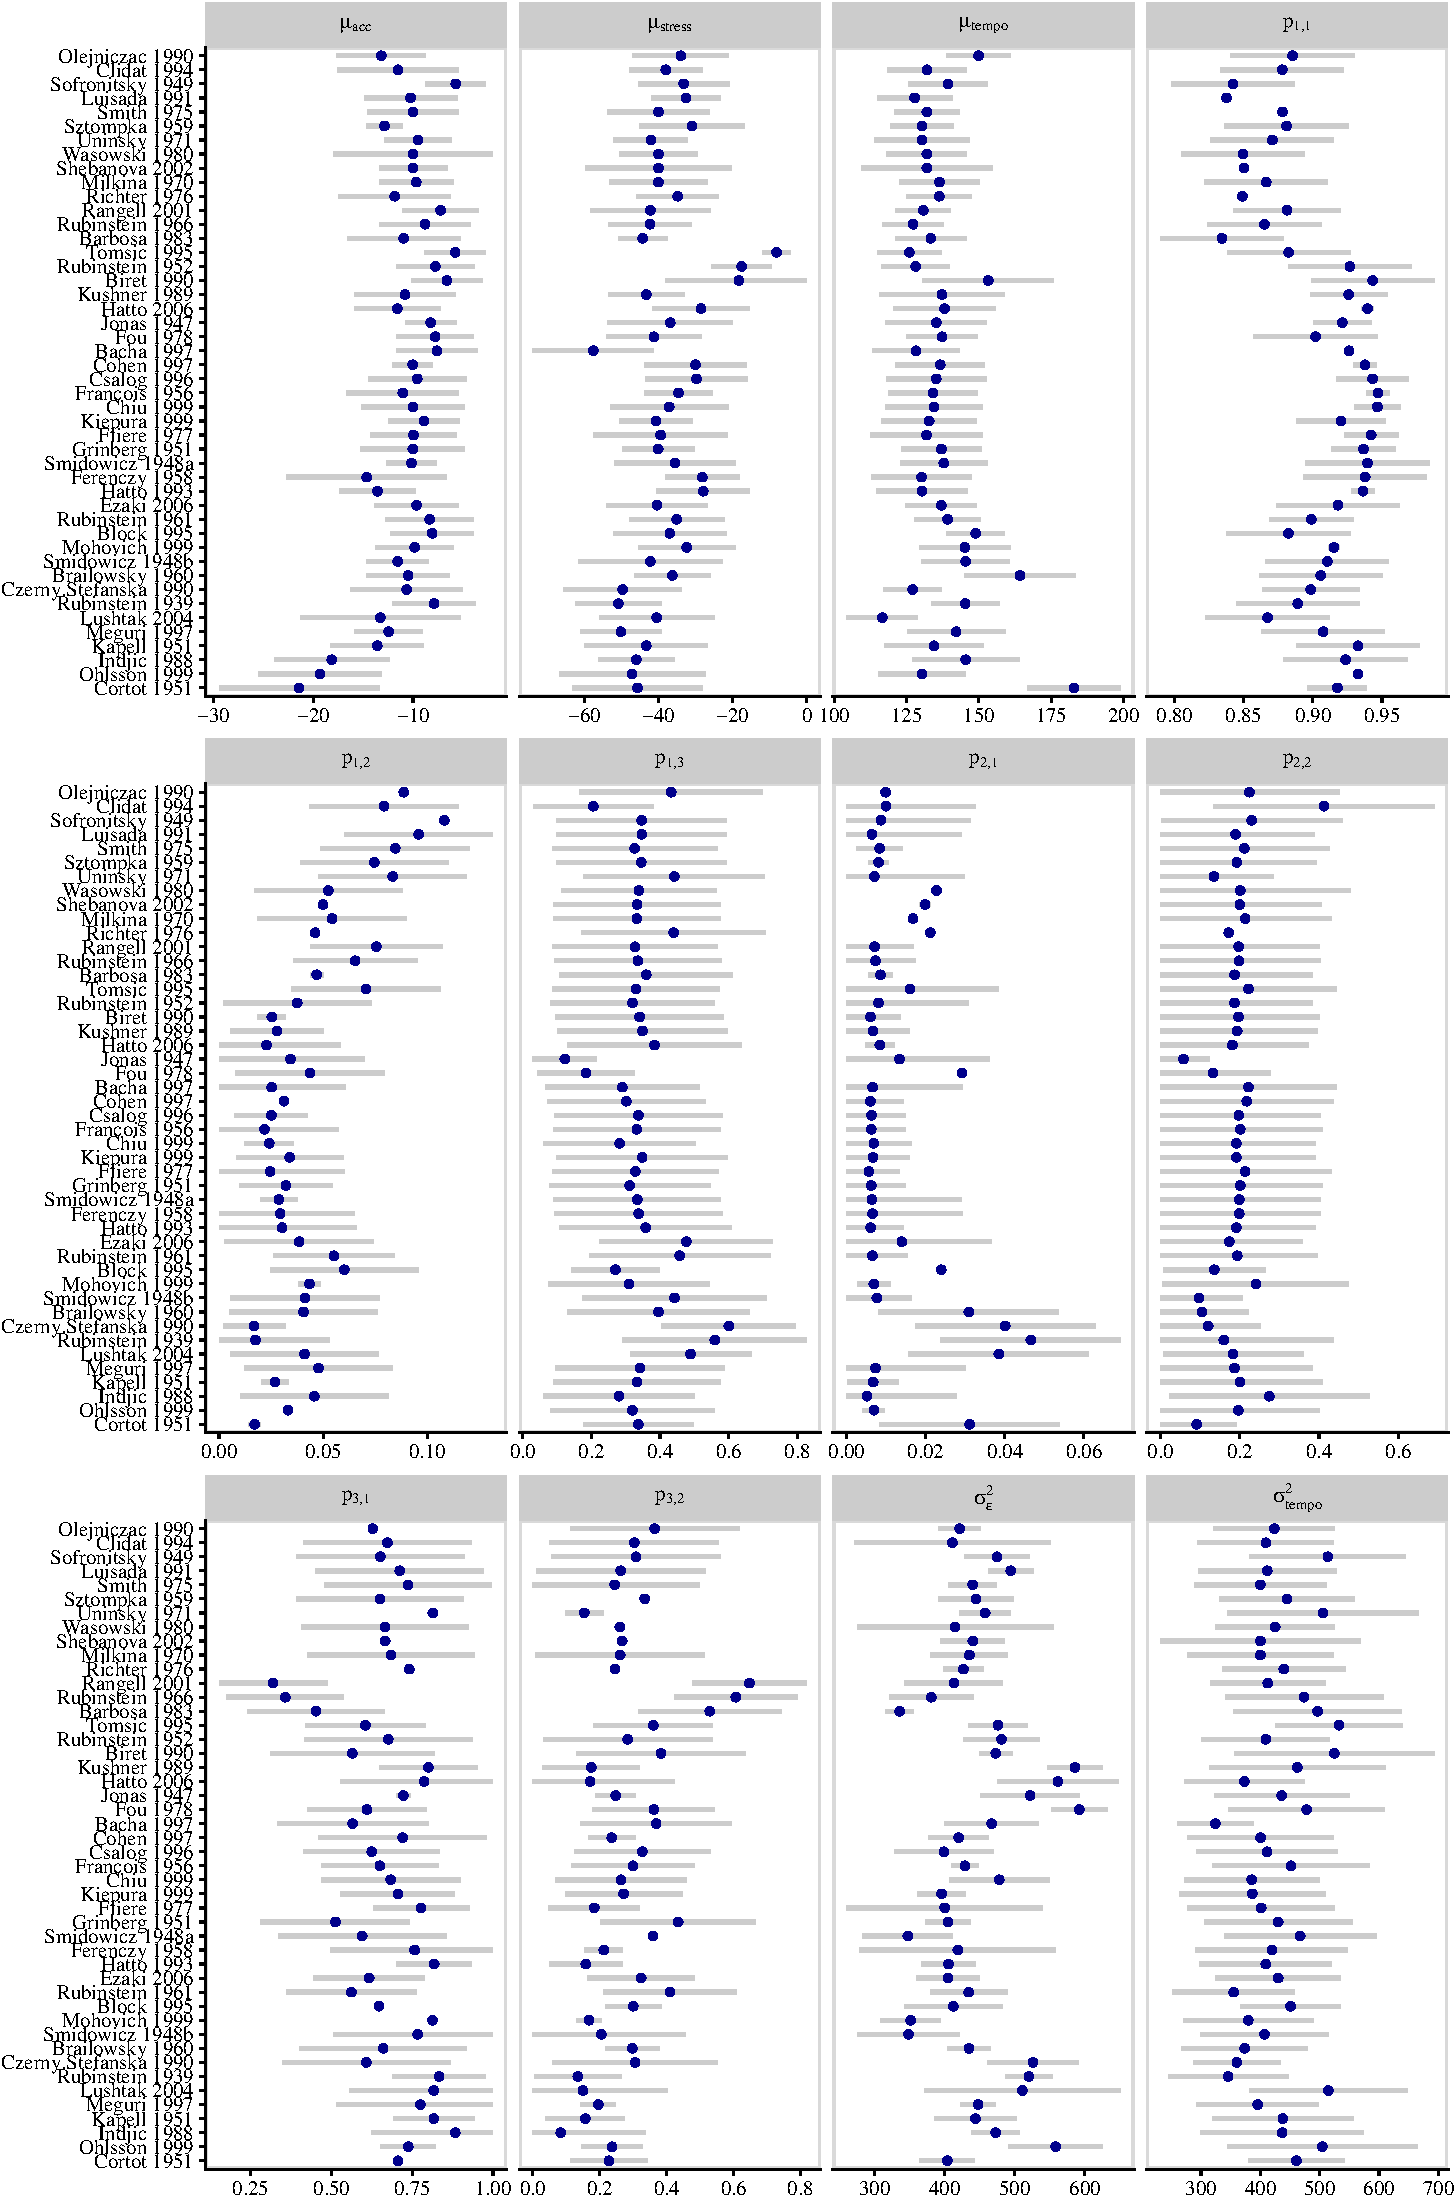
\includegraphics[width=5.333in,height=8in]{gfx/confidence-intervals-1} 

}

\caption{Confidence intervals for all parameters based on the observed Fisher information.}\label{fig:confidence-intervals}
\end{figure}

\autoref{sec:analys-chop-mazurka} of the manuscript includes parameter
estimates for some of the recordings in our data set. In order to
quantify uncertainty and compare the estimates, this section graphically
displays all parameter estimates in \autoref{fig:confidence-intervals}.
The recordings are sorted in the same order as in \autoref{fig:dmats} in
the main document, so some of the conclusions about groupings are
readily apparent. The bars indicating measures of uncertainty are
derived form the observed Fisher information from the optimization
routine. However, it's not entirely clear what these mean. For one, they
ignore any uncertainty in the state sequence (see
\autoref{fig:posterior-richter-plot} some notion of the scale of this
uncertainty). They also depend on identifiability, the priors, and the
approximation to the posterior. Producing the MAP depends on the
approximation accuracy at the MAP, but producing the Hessian needs that
as well as the accuracy of about \(5p^2\) additional function
evaluations. And because we need the inverse, any inaccuracies could
explode. The length of the confidence interval for parameter \(j\) is
given by \(4\sqrt{(\widehat{I})^{-1}_{jj}}\) and so these would have
roughly 95\% coverage. For any parameters that are unidentified, the
width of the band is the maximum over all performances for the same
parameter. However, short of performing a fully-Bayesian analysis, we
would hesitate to attach much certainty to these metrics of uncertainty.

\hypertarget{distance-matrix-from-raw-data}{%
\section{Distance matrix from raw
data}\label{distance-matrix-from-raw-data}}

In \autoref{sec:clust-music-perf} of the manuscript, we present results
for grouping performances using the low-dimensional vector of
performance specific parameters learned for our model. An alternative
approach is to simply use the raw data, in this case, 231 individual
note-by-note instantaneous speeds measured in beats per minute. In
\autoref{fig:raw-data-clusters} we show the result of this analysis. A
comparison between this clustering and that given by our model is
discussed in some detail in the manuscript.

\begin{figure}[b]

{\centering 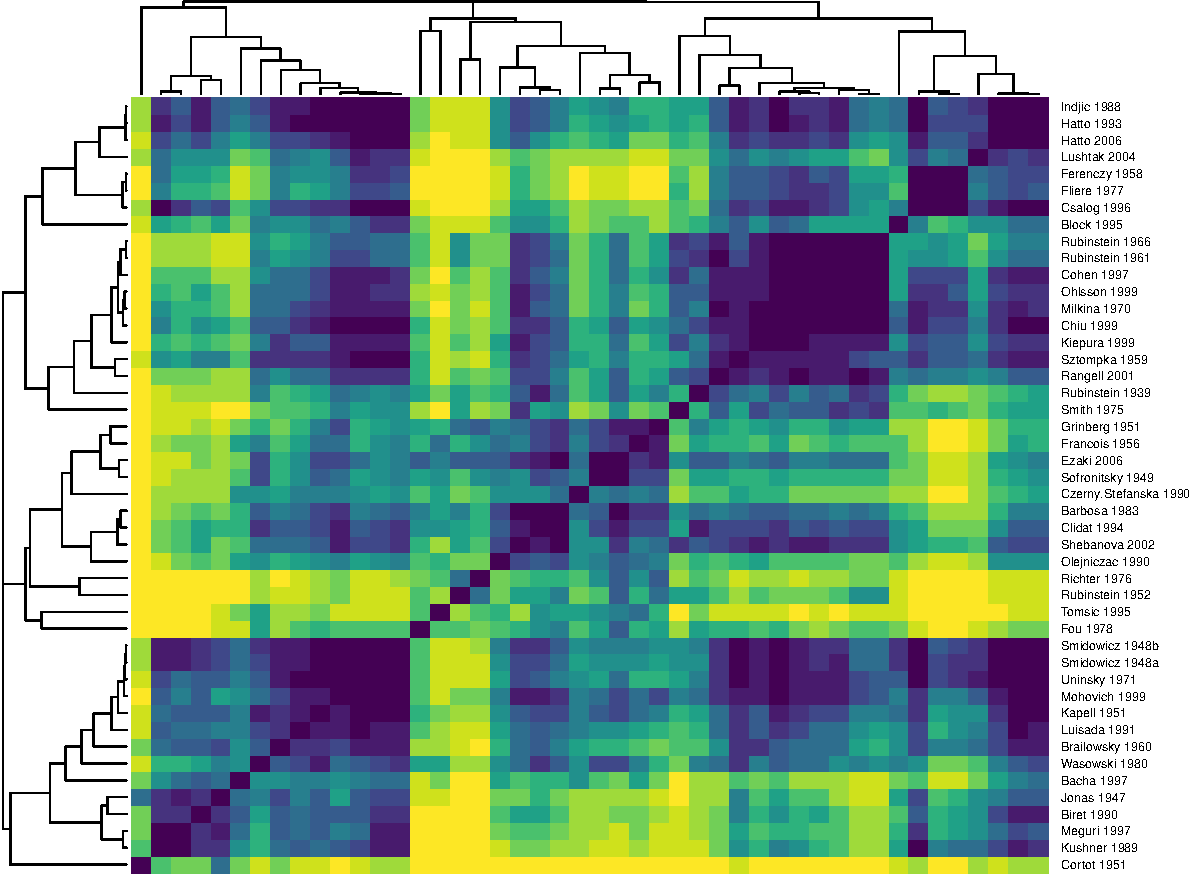
\includegraphics[width=4in]{gfx/raw-data-clusters-1} 

}

\caption{This figure presents a heatmap and hierarchical clustering based only on the note-by-note onset timings for each of the 46 recordings.}\label{fig:raw-data-clusters}
\end{figure}

\hypertarget{plotting-performances}{%
\section{Plotting performances}\label{plotting-performances}}

\autoref{sec:clust-music-perf} of the manuscript discusses 7 groups of
recordings. Figures \ref{fig:clust-1} to \ref{fig:clust-7} display the
note-by-note tempos along with the inferred interpretive decisions for
all performances based on this grouping.

The first group (\autoref{fig:clust-1} indicated as \(\circ\) in
\autoref{fig:pca}) corresponds to reasonably staid performances. This
group is the largest and corresponds to the block from Cohen to
Brailowsky in \autoref{fig:dmats}. In this group, the emphasis state is
rarely visited with the performer tending to stay in the constant tempo
state with periods of slowing down at the ends of phrases. Acceleration
is almost never used. Furthermore, these performances have relatively
slow average tempos, and not much difference between the A and B
sections. Joyce Hatto's recording in \autoref{fig:archetypal} is typical
of this group

\begin{figure}

{\centering 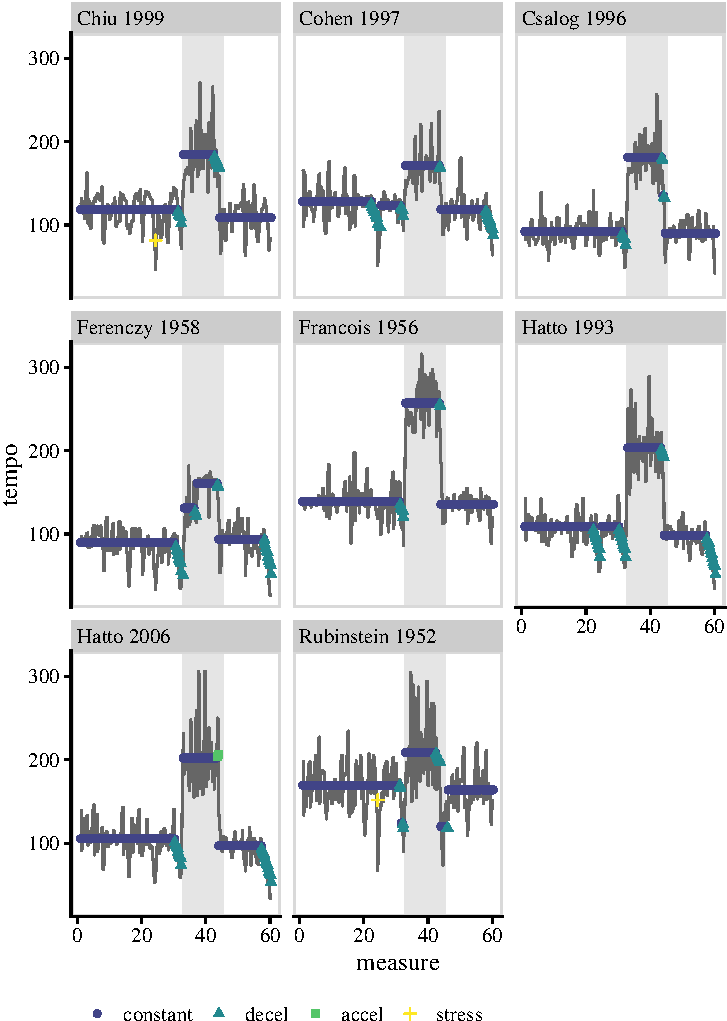
\includegraphics{gfx/clust-1-1} 

}

\caption{Performances in the first group}\label{fig:clust-1}
\end{figure}

Recordings in the fourth group (\autoref{fig:clust-4}, \(\oplus\) in
\autoref{fig:pca}) are those in the upper right of \autoref{fig:dmats},
from Olejniczac to Richter. These recordings tend to transition quickly
between states, especially constant tempo and slowing down accompanied
by frequent transitory emphases. The probability of remaining in state 1
is the lowest while the probability of entering state 2 from state 1 is
the highest. The acceleration state is rarely visited. Four of the most
similar performances are in this group along with Richter's 1976
recording.

\begin{figure}

{\centering 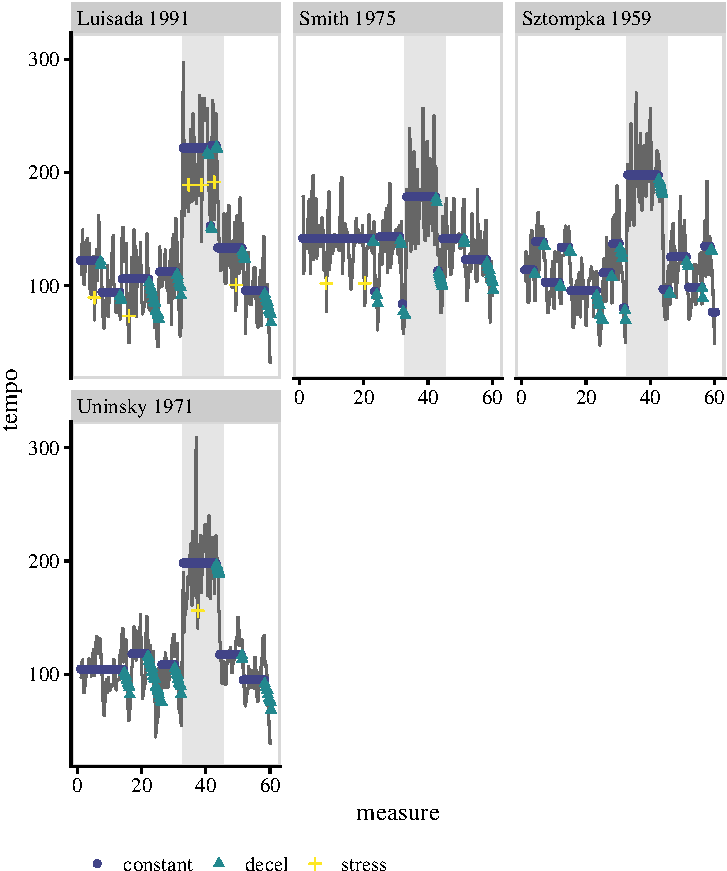
\includegraphics{gfx/clust-4-1} 

}

\caption{Performances in the fourth group.}\label{fig:clust-4}
\end{figure}

The three performances in group six (\autoref{fig:clust-6}, \(\bullet\)
in \autoref{fig:pca}) are actually quite like others, but with small
exceptions. Biret's 1990 performance is very much like those in group 1,
but with a much larger contrast between tempos in the A and B sections.
The recording by Rubinstein in 1952 is similar, though with a faster A
section that has less contrast with the B section. Tomsic's 1995
performance is actually most similar to those in group three
(\(\mathrlap{+}\times\)), but played much faster and with a large
\(\sigma^2_\epsilon\).

\begin{figure}

{\centering 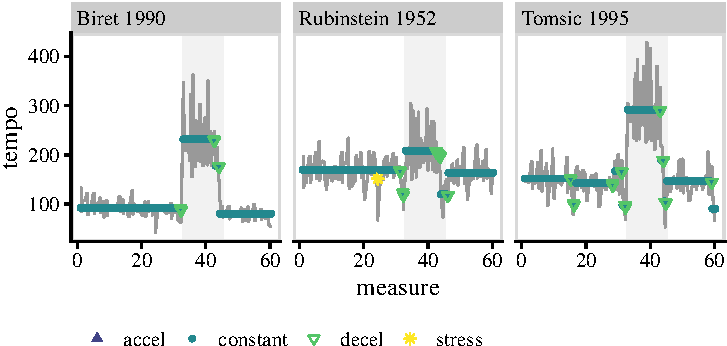
\includegraphics{gfx/clust-6-1} 

}

\caption{Performances in the sixth group.}\label{fig:clust-6}
\end{figure}

The remaining performances are displayed in Figures
\ref{fig:clust-2}--\ref{fig:clust-7}, with the exception of Cortot's
performance in the manuscript.

\begin{figure}

{\centering 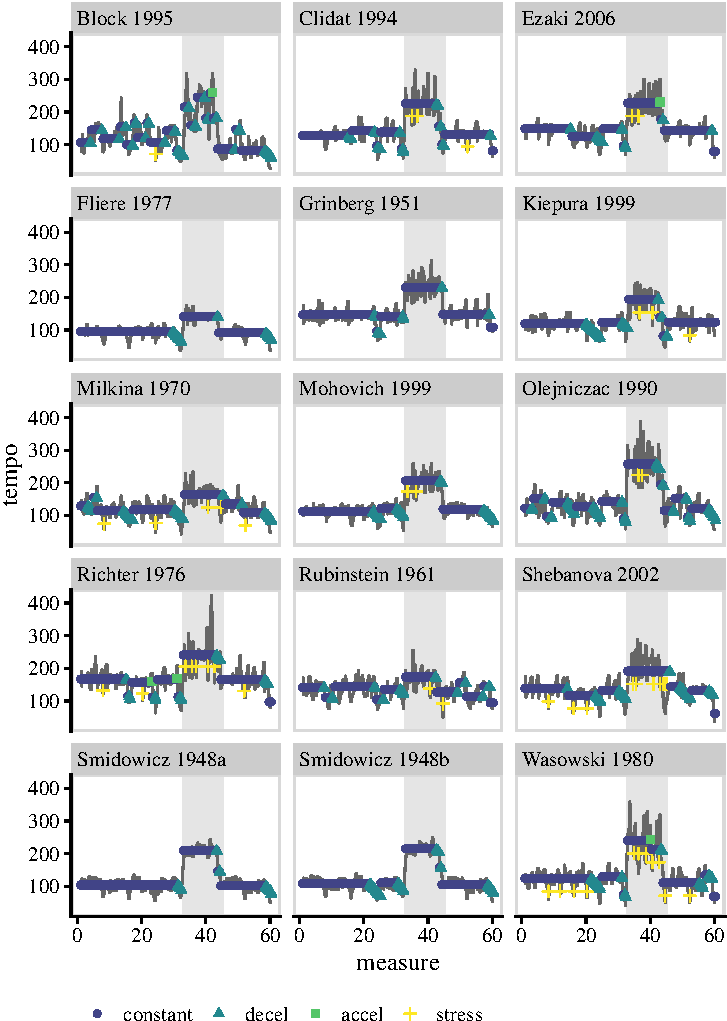
\includegraphics{gfx/clust-2-1} 

}

\caption{Performances in the second group.}\label{fig:clust-2}
\end{figure}

\begin{figure}

{\centering 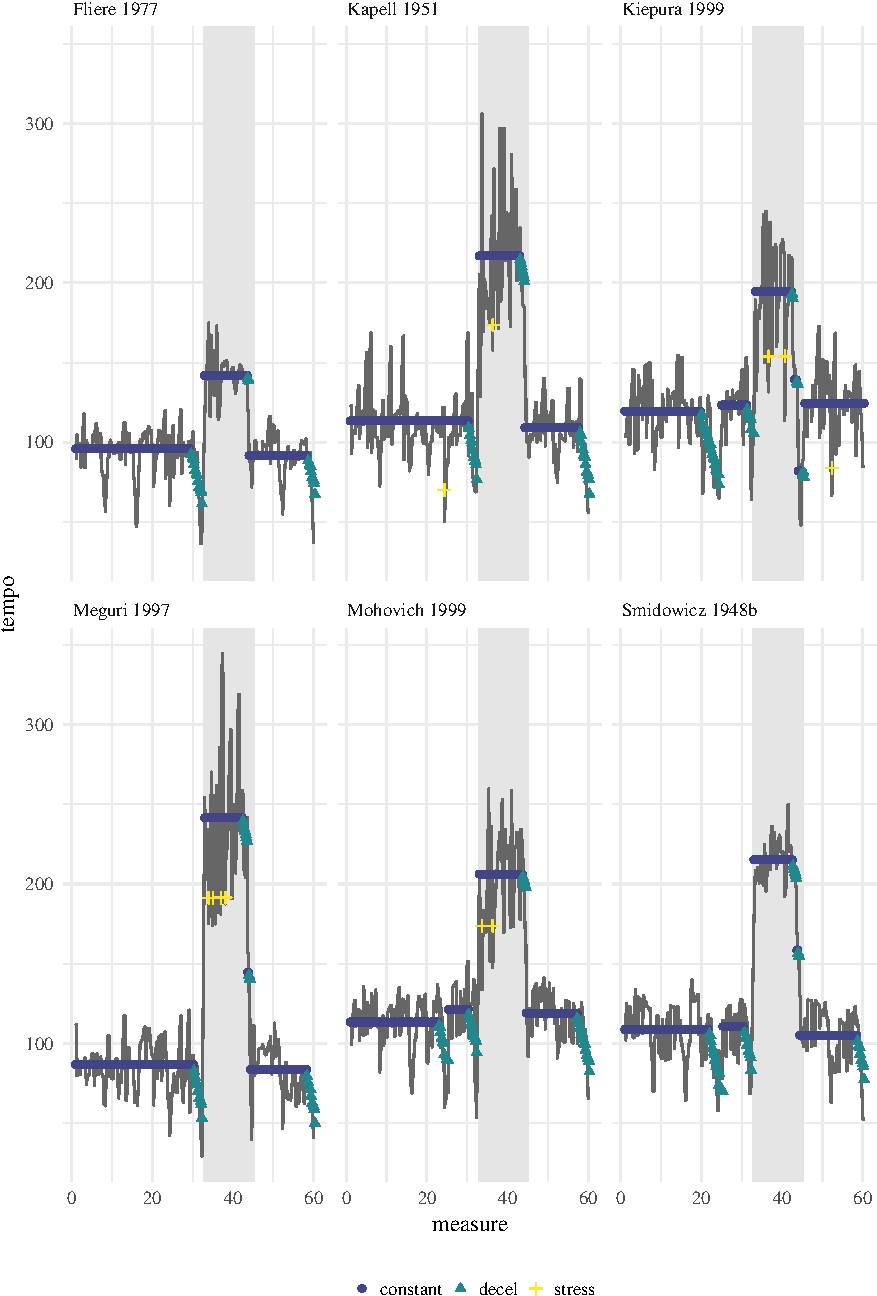
\includegraphics{gfx/clust-3-1} 

}

\caption{Performances in the third cluster.}\label{fig:clust-3}
\end{figure}

\begin{figure}

{\centering 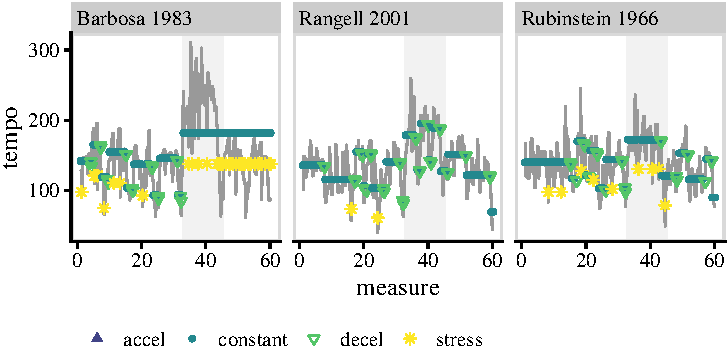
\includegraphics{gfx/clust-5-1} 

}

\caption{Performances in the fifth group.}\label{fig:clust-5}
\end{figure}

\begin{figure}

{\centering 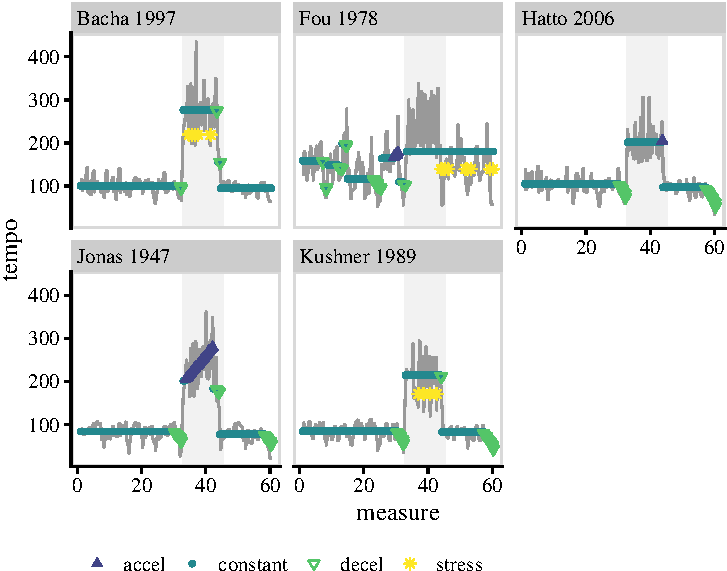
\includegraphics{gfx/clust-7-1} 

}

\caption{Performances in the seventh group.}\label{fig:clust-7}
\end{figure}

\hypertarget{distribution-over-states}{%
\section{Distribution over states}\label{distribution-over-states}}

To examine the stability of the \autoref{alg:dpf}, we examined all the
potential paths for Richter's 1976 recording. Here, we saved the most
likely 10,000 paths and their weights (rather than only the most likely
path). \autoref{fig:posterior-richter-plot} shows the marginal
(posterior) probability of being in a particular state for each note.
While the paper uses the most likely \emph{path}, this figure is
marginal in the sense that a particular note/state combination will have
high probability when many paths visited that note/state. But, the most
likely path may not have used that same note/state combination.
Nonetheless, there appears to be consensus for many of the notes. The
most obviously difficult notes are those near measures 10 and 50. In
both cases, the most likely path (\autoref{fig:richter} in the main
text) used the stress state, which exceeds 50\% posterior probability
here.

\begin{figure}

{\centering 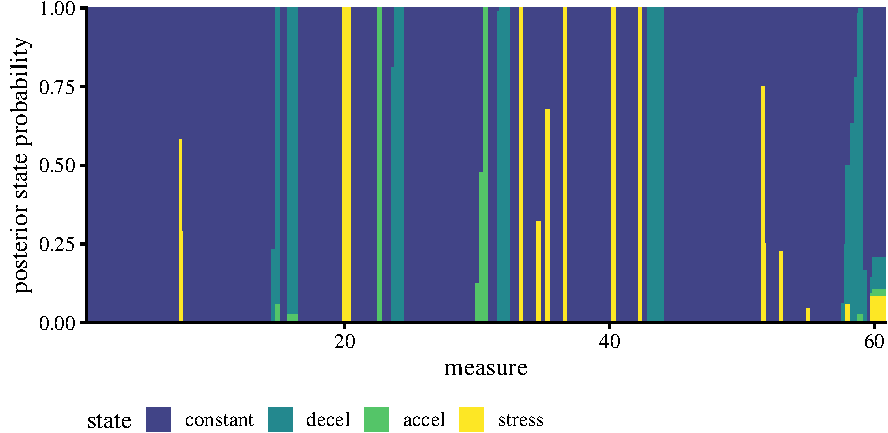
\includegraphics[height=2in]{gfx/posterior-richter-plot-1} 

}

\caption{Distribution over potentitial states for Richter's 1976 recording.}\label{fig:posterior-richter-plot}
\end{figure}

\hypertarget{multiplicative-tempo-changes}{%
\section{Multiplicative tempo
changes}\label{multiplicative-tempo-changes}}

\begin{figure}

{\centering 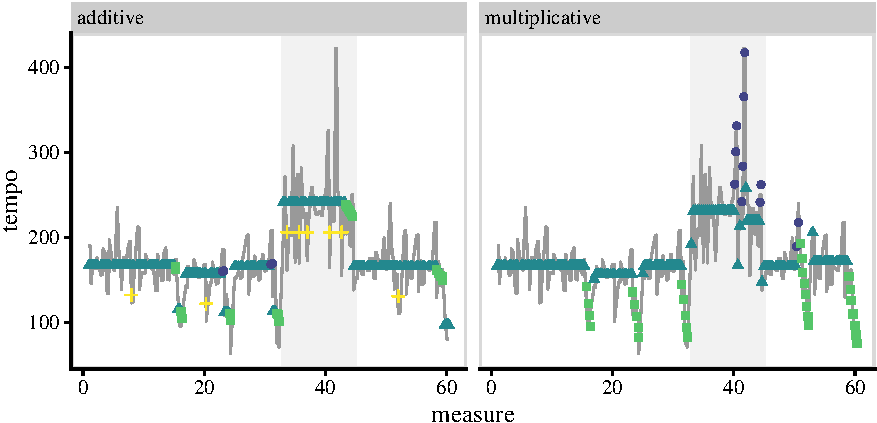
\includegraphics[width=5in]{gfx/multiplicative-model-1} 

}

\caption{Additive and multiplicative models for Richter's 1976 performance. The multiplicative model fits quite well, but is less likely to visit the stress state.}\label{fig:multiplicative-model}
\end{figure}

While an additive state space model is relatively easy to understand,
some music theorists \citep[for example]{Mead2007} have argued that
musicians make multiplicative tempo adjustments. That is, it is the
ratio between the tempo of the current note and that of the previous
note rather than their difference that is important. Such a conception
is fundamental to musical notation (quarter notes, eighth notes, etc)
and frequently used to specify tempo changes within a piece of music,
such as with \halfnote~=~\quarternote~to indicate that the next section
should be played at half the previous tempo.

Rather than the linear switching model described in
\autoref{sec:materials-methods}, we examined the following
multiplicative version: \begin{equation}
  \begin{aligned}
    x_1 &\sim \textrm{lognormal}(x_0,\ P_0),\\
    \frac{x_{i+1}}{x_i} &= (1-\mu(s_i)) \eta_i, 
    & \eta_i &\sim \textrm{lognormal}(0,\ Q(s_i)),\\
    y_i&= c(s_i) +x_i + \epsilon_i, & \epsilon_i &\sim N(0,\ G(s_i)).
  \end{aligned}
\end{equation} Here, \(\mu(s_i)\) is 0 in the constant tempo or emphasis
states and controls the magnitude of acceleration or deceleration in the
other states. To complete the model,
\(G=\sigma^2_\epsilon + \sigma^2_{stress}I(s_i=4)\) while
\(Q = \sigma^2_{acc}\) in states 2 or 3 and 0 otherwise. To make this
model easier to compute, we transform by examining the log of the
transition equation and exponentiating the hidden continuous state in
the measurement equation. Likelihood evaluation is then performed with
the extended Kalman filter (EKF). The EKF is essentially the Kalman
filter applied to the first-order Taylor series expansion of any
non-linear components around our current predictions of them. For this
model, we have \begin{equation}
  \begin{aligned}
    \log(x_1) &\sim N(x_0,\ P_0),\\
    \log(x_{i+1}) &= \log(x_i) + \log(1-\mu(s_i)) + \log(\eta_i), 
    & \log(\eta_i) &\sim N(0,\ Q(s_i)),\\
    y_i&= c(s_i) +\exp(\varx_i) + \exp(\varx_i)x_i + \epsilon_i, & \epsilon_i &\sim N(0,\ G(s_i)),
  \end{aligned}
\end{equation} where \(\varx_i\) is the estimate of
\(E\left[x_i \given y_1,\ldots y_{i-1}\right]\).

We estimated this same model on the entire dataset and performed
principal component analysis on the resulting parameters (see also
\autoref{sec:clust-music-perf} of the manuscript).
\autoref{fig:multiplicative-model} shows the inferred performance
decisions for Richter's 1976 performance from both the linear and
multiplicative models. Both seem to fit the data quite well. There are
three slight differences between the inferences. First, in the B
section, the multiplicative model uses the acceleration state more than
the additive model does. Second, the multiplicative model avoids the
stress state, and this behavior is reflected in a higher probability of
remaining in the constant tempo state. Third, the perioods of slowing
down at the ends of phrases are better explained by the multiplicative
model.

\begin{figure}

{\centering 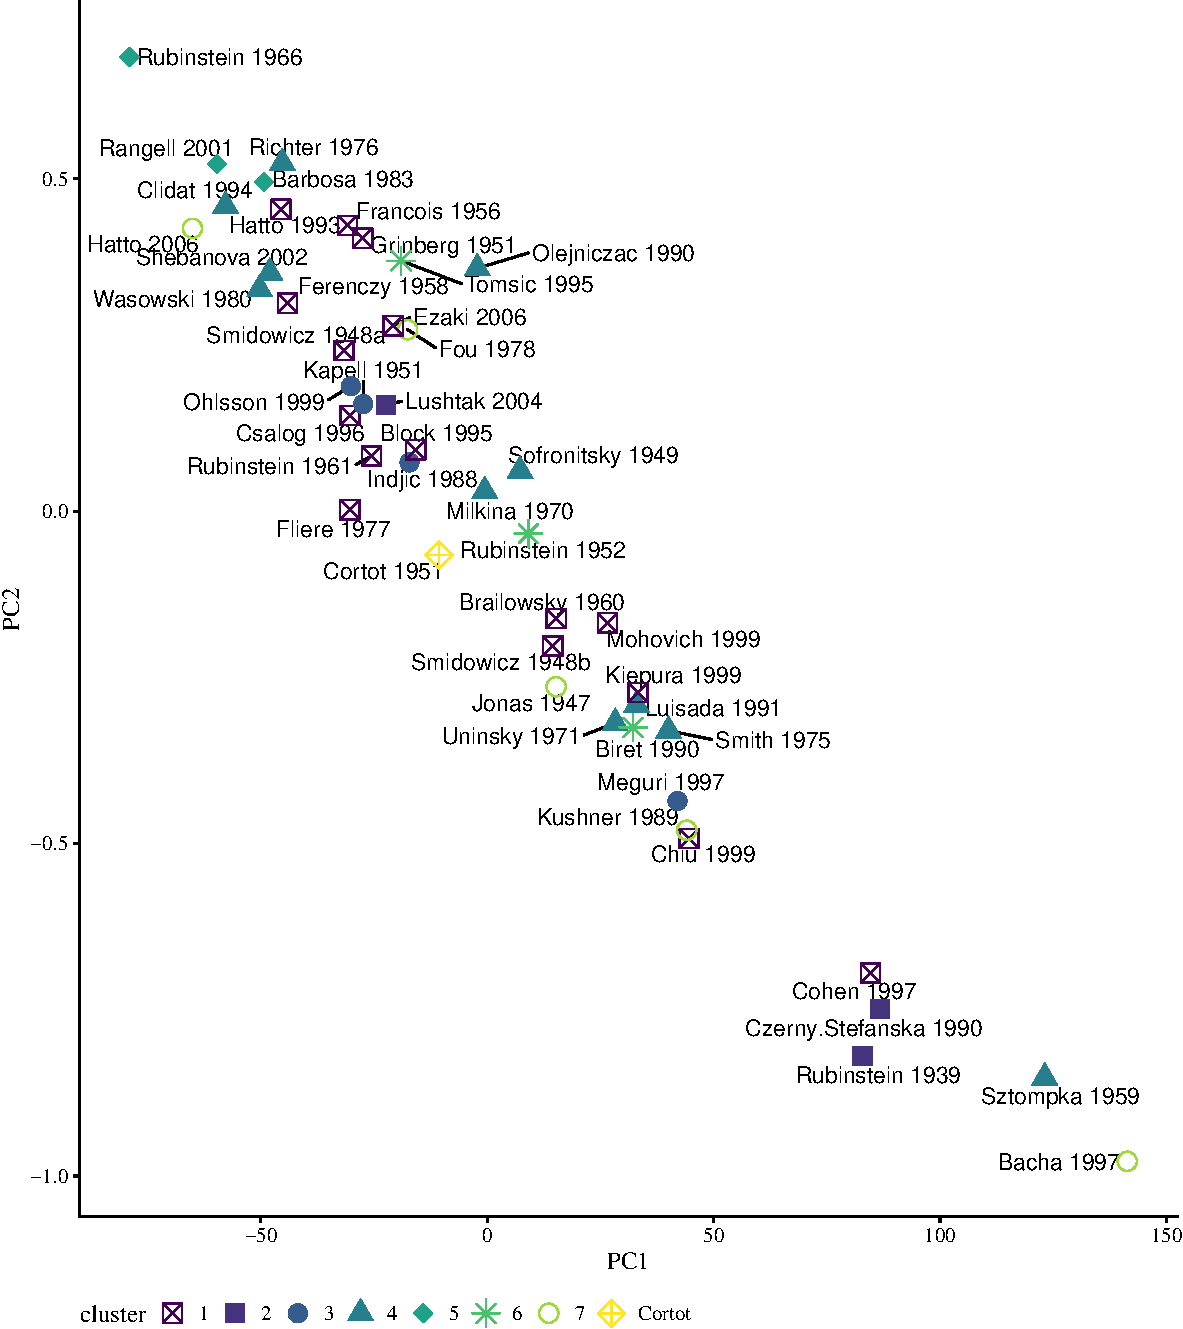
\includegraphics[width=5in]{gfx/mult-par-clusts-1} 

}

\caption{The first two principal components based on parameter estimates from the multiplicative model. The groupings (color and point type) are the same as those from the linear model.}\label{fig:mult-par-clusts}
\end{figure}

The percent of variance explained by the first two principal components
is 99\%. The first factor loads completely on \(\sigma^2_{\epsilon}\)
while the second loads on \(\mu_{\textrm{stress}}\). So, while this
model can explain individual performances quite well, it is much less
able to provide musically meaningful distinctions between performances.
While the interpretation for Richter's performance seems quite
reasonable under this model, other performances are much less
reasonable.

\hypertarget{alternative-prior-distributions}{%
\section{Alternative prior
distributions}\label{alternative-prior-distributions}}

Following the recommendations of an anonymous referee, we reestimated
the model under some alternative prior distributions. These
distributions are shown in \autoref{tab:morepriors}. Returning to
Richter's recording, we used inverse gamma and uniform distributions for
the variance parameters to allow heavier tails. We also looked at
uniform distributions on the transition probabilities and a prior which
requires the observation variance, \(\sigma^2_\epsilon\) to be smaller.

Apart from the ``smaller observation variance'' setting, these different
specifications do not have a dramatic effect: the fit to the data
remains similar both quantitatively (as measured by RMSE and negative
loglikelihood, see \autoref{tab:prior-mses}) and qualitatively (as
determined by examining the inferred performance in
\autoref{fig:alternative-priors}).

The prior modes are important for some parameters to avoid
non-identifiability, and occasionally, as described in the manuscript,
to enforce more musically meaningful switching behaviors. On the other
hand, the prior tail shape is not particularly important here because
we're estimating posterior modes rather than performing a full Bayesian
analysis with accompanying credible intervals.

\begin{table}[t]
    \caption{Informative prior distributions for the music model}
  \label{tab:morepriors}
  \centering
  \begin{tabular}{@{}rcccc@{}}
    \toprule
    Parameter & \phantom{a} & Original & Inverse Gamma \\
    \midrule
    $\sigma^2_{\epsilon}$ & $\sim$ & Gamma$(40,\ 10)$ & IG$(42,16400)$\\
    $\mu_{\textrm{tempo}}$ & $\sim$ & Gamma$\left(\frac{\overline{Y}^2}{100},\ \frac{100}{\overline{Y}}\right)$ & IG$\left(\frac{\overline{Y}^2}{100}+2, \overline{Y}(\frac{\overline{Y}^2}{100}+1)\right)$\\
    $-\mu_{\textrm{acc}} $ & $\sim$ & Gamma$(15,\ 2/3)$ & IG(17, 160)\\
    $-\mu_{\textrm{stress}} $ & $\sim$ & Gamma$(20,\ 2)$ & IG(22, 840\\
    $\sigma^2_{\textrm{tempo}} $ & $\sim$ & Gamma$(40,\ 10)$ & IG$(42,16400)$\\
    $\sigma^2_{\textrm{acc}} $ & $=$ & 1 &  1\\
    $\sigma^2_{\textrm{stress}} $ & $=$ & 1 & 1\\
    $p_{1,\cdot}$ & $\sim$ & Dirichlet$(85,\ 5,\ 2,\ 8)$& Dirichlet$(85,\ 5,\ 2,\ 8)$ \\
    $p_{2,\cdot}$ & $\sim$ & Dirichlet$(4,\ 10,\ 1,\ 0)$& Dirichlet$(4,\ 10,\ 1,\ 0)$ \\
    $p_{3,\cdot}$ & $\sim$ & Dirichlet$(5,\ 3,\ 7,\ 0)$& Dirichlet$(5,\ 3,\ 7,\ 0)$ \\
    \midrule
    Parameter & \phantom{a} & Smaller $\sigma^2_\epsilon$ &
    Uniform Variances & Uniform Probabilities\\
    \midrule
    $\sigma^2_{\epsilon}$ & $\sim$ & Gamma$(20,\ 10)$ & 1 & Gamma$(20,\ 10)$ \\
    $\mu_{\textrm{tempo}}$ & $\sim$ & Gamma$\left(\frac{\overline{Y}^2}{100},\ \frac{100}{\overline{Y}}\right)$ & Gamma$\left(\frac{\overline{Y}^2}{100},\ \frac{100}{\overline{Y}}\right)$ & Gamma$\left(\frac{\overline{Y}^2}{100},\ \frac{100}{\overline{Y}}\right)$ \\
    $-\mu_{\textrm{acc}} $ & $\sim$ & Gamma$(15,\ 2/3)$ & Gamma$(15,\ 2/3)$ & Gamma$(15,\ 2/3)$\\
    $-\mu_{\textrm{stress}} $ & $\sim$ & Gamma$(20,\ 1)$ & Gamma$(20,\ 2)$ & Gamma$(20,\ 2)$ \\
    $\sigma^2_{\textrm{tempo}} $ & $\sim$ & Gamma$(40,\ 10)$ & 1 & Gamma$(40,\ 10)$\\
    $\sigma^2_{\textrm{acc}} $ & $=$ & 1 &  1 & 1\\
    $\sigma^2_{\textrm{stress}} $ & $=$ & 1 & 1 & 1\\
    $p_{1,\cdot}$ & $\sim$ & Dirichlet$(85,\ 5,\ 2,\ 8)$& Dirichlet$(85,\ 5,\ 2,\ 8)$& 1 \\
    $p_{2,\cdot}$ & $\sim$ & Dirichlet$(4,\ 10,\ 1,\ 0)$& Dirichlet$(4,\ 10,\ 1,\ 0)$& 1 \\
    $p_{3,\cdot}$ & $\sim$ & Dirichlet$(5,\ 3,\ 7,\ 0)$& Dirichlet$(5,\ 3,\ 7,\ 0)$& 1 \\
    \bottomrule
  \end{tabular}
\end{table}

\begin{figure}

{\centering 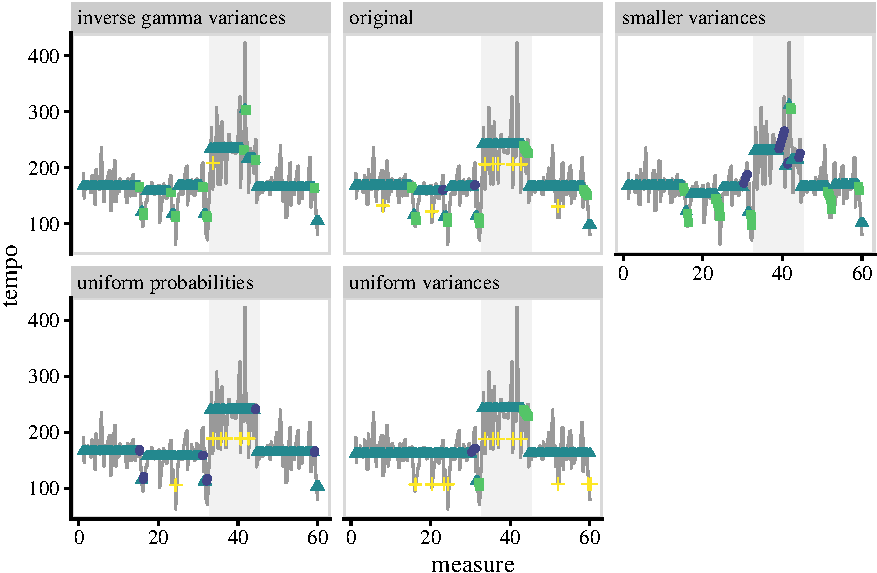
\includegraphics[width=5in]{gfx/alternative-priors-1} 

}

\caption{Inferred state sequence for Richter's 1976 recording under alternative prior specifications.}\label{fig:alternative-priors}
\end{figure}

\begin{table}

\caption{\label{tab:prior-mses}For each of the different prior distributions, we report the MSE between the estimated performer intentions from the model and the true performance as well as the negative log likelihood.}
\centering
\begin{tabular}[t]{lrrr}
\toprule
prior & rmse & negative log likelihood & $\sigma_{\epsilon}$\\
\midrule
inverse gamma variances & 28.57 & -5.20 & 20.66\\
original & 29.31 & -5.10 & 19.24\\
smaller variances & 26.77 & -5.10 & 20.01\\
uniform probabilities & 30.54 & -5.06 & 21.27\\
uniform variances & 31.05 & -5.15 & 23.56\\
\bottomrule
\end{tabular}
\end{table}

\begin{table}

\caption{\label{tab:posterior-ests}For each of the different prior distributions, we report the estimated parameter values.}
\centering
\resizebox{\linewidth}{!}{
\begin{tabular}[t]{lrrrrr}
\toprule
  & original & smaller variances & inverse gamma variances & uniform variances & uniform probabilities\\
\midrule
$\sigma^2_{\epsilon}$ & 426.70 & 370.37 & 400.36 & 452.49 & 555.29\\
$\mu_{\textrm{tempo}}$ & 136.33 & 167.65 & 166.55 & 133.34 & 135.69\\
$\mu_{\textrm{acc}}$ & -11.84 & -23.55 & -6.44 & -10.02 & -7.74\\
$\mu_{\textrm{stress}}$ & -34.82 & -16.76 & -24.75 & -54.16 & -50.89\\
$\sigma^2_{\textrm{tempo}}$ & 439.38 & 451.58 & 400.57 & 406.50 & 320.17\\
$p_{11}$ & 0.85 & 0.94 & 0.91 & 0.90 & 0.93\\
$p_{12}$ & 0.05 & 0.03 & 0.05 & 0.02 & 0.01\\
$p_{22}$ & 0.74 & 0.46 & 0.52 & 0.68 & 0.85\\
$p_{31}$ & 0.44 & 0.22 & 0.30 & 0.29 & 0.74\\
$p_{13}$ & 0.02 & 0.01 & 0.01 & 0.01 & 0.03\\
$p_{21}$ & 0.25 & 0.47 & 0.45 & 0.26 & 0.08\\
$p_{32}$ & 0.17 & 0.04 & 0.20 & 0.13 & 0.15\\
\bottomrule
\end{tabular}}
\end{table}


\clearpage

\bibliographystyle{mybibsty}
\bibliography{chopinrefs.bib}

\end{document}
